\documentclass[%
 reprint,
%superscriptaddress,
%groupedaddress,
%unsortedaddress,
%runinaddress,
%frontmatterverbose, 
%preprint,
%showpacs,preprintnumbers,
%nofootinbib,
%nobibnotes,
%bibnotes,
 amsmath,amssymb,
 aps,
%pra,
%prb,
%rmp,
%prstab,
%prstper,
%floatfix,
]{revtex4-1}

\usepackage{graphicx}% Include figure files
\usepackage{dcolumn}% Align table columns on decimal point
\usepackage{bm}% bold math
%\usepackage{hyperref}% add hypertext capabilities
%\usepackage[mathlines]{lineno}% Enable numbering of text and display math
%\linenumbers\relax % Commence numbering lines

%\usepackage[showframe,%Uncomment any one of the following lines to test 
%%scale=0.7, marginratio={1:1, 2:3}, ignoreall,% default settings
%%text={7in,10in},centering,
%%margin=1.5in,
%%total={6.5in,8.75in}, top=1.2in, left=0.9in, includefoot,
%%height=10in,a5paper,hmargin={3cm,0.8in},
%]{geometry}

\usepackage{cmap} % Поиск в PDF
\usepackage[T2A]{fontenc} % Кодировка
\usepackage[utf8]{inputenc} % Кодировка исходного текста
\usepackage[english, russian]{babel} % Локализация и переносы
\frenchspacing % Более тонкая настройка пробелов 
\usepackage{multirow}
\usepackage[warn]{mathtext}
\usepackage{amssymb}
\usepackage{ dsfont }
\usepackage{ textcomp }
\usepackage{ mathrsfs }

% Переопределение англоязычного начертания каппа, фи и эпсилон, 
% а также знаков сравнения
\renewcommand{\epsilon}{\ensuremath{\varepsilon}}
\renewcommand{\phi}{\ensuremath{\varphi}} 
\renewcommand{\kappa}{\ensuremath{\varkappa}}
\renewcommand{\le}{\ensuremath{\leslant}}
\renewcommand{\leq}{\ensuremath{\leqslant}}
\renewcommand{\ge}{\ensuremath{\geslant}}
\renewcommand{\geq}{\ensuremath{\geqslant}}
\renewcommand{\emptyset}{\ensuremath{\varnothing}}

\usepackage{textcomp} 
\usepackage{indentfirst} % Красная строка
\usepackage{amsmath} % Текст в формулах
\usepackage{graphicx} % Графика
\DeclareGraphicsExtensions{.pdf,.png,.jpg}
\usepackage{pgfplots}
\pgfplotsset{compat=1.13}

%\usepackage{times}

\begin{document}

\title{Экспериментальная проверка закона Видемана-Франца}
\thanks{11.8}

\author{Иван Едигарьев}
\affiliation{
 Московский Физико-Технический Институт\\
 Факультет Общей и Прикладной Физики, 526т\\
}
%\date{\today}

\begin{abstract}
Целью работы является экспериментальное определение величины постоянной Лоренца
$L~=~\kappa /(\sigma T)$ при комнатной температуре для нескольких распространенных металлов и сплавов: меди, латуни, алюминия, дюралюминия.

\end{abstract}

\pacs{Valid PACS appear here}

\maketitle

\begin{enumerate}

\item 
\textbf{Измерение вольт-амперной характеристики образца для определения сопротивления}\\
По показаниям вольтметра и амперметра снимем вольт-амперную характеристику.
По линейной зависимости $U(I) = U_0 + RI$ определим сопротивление образца $R$:
\begin{figure}[h]
\center{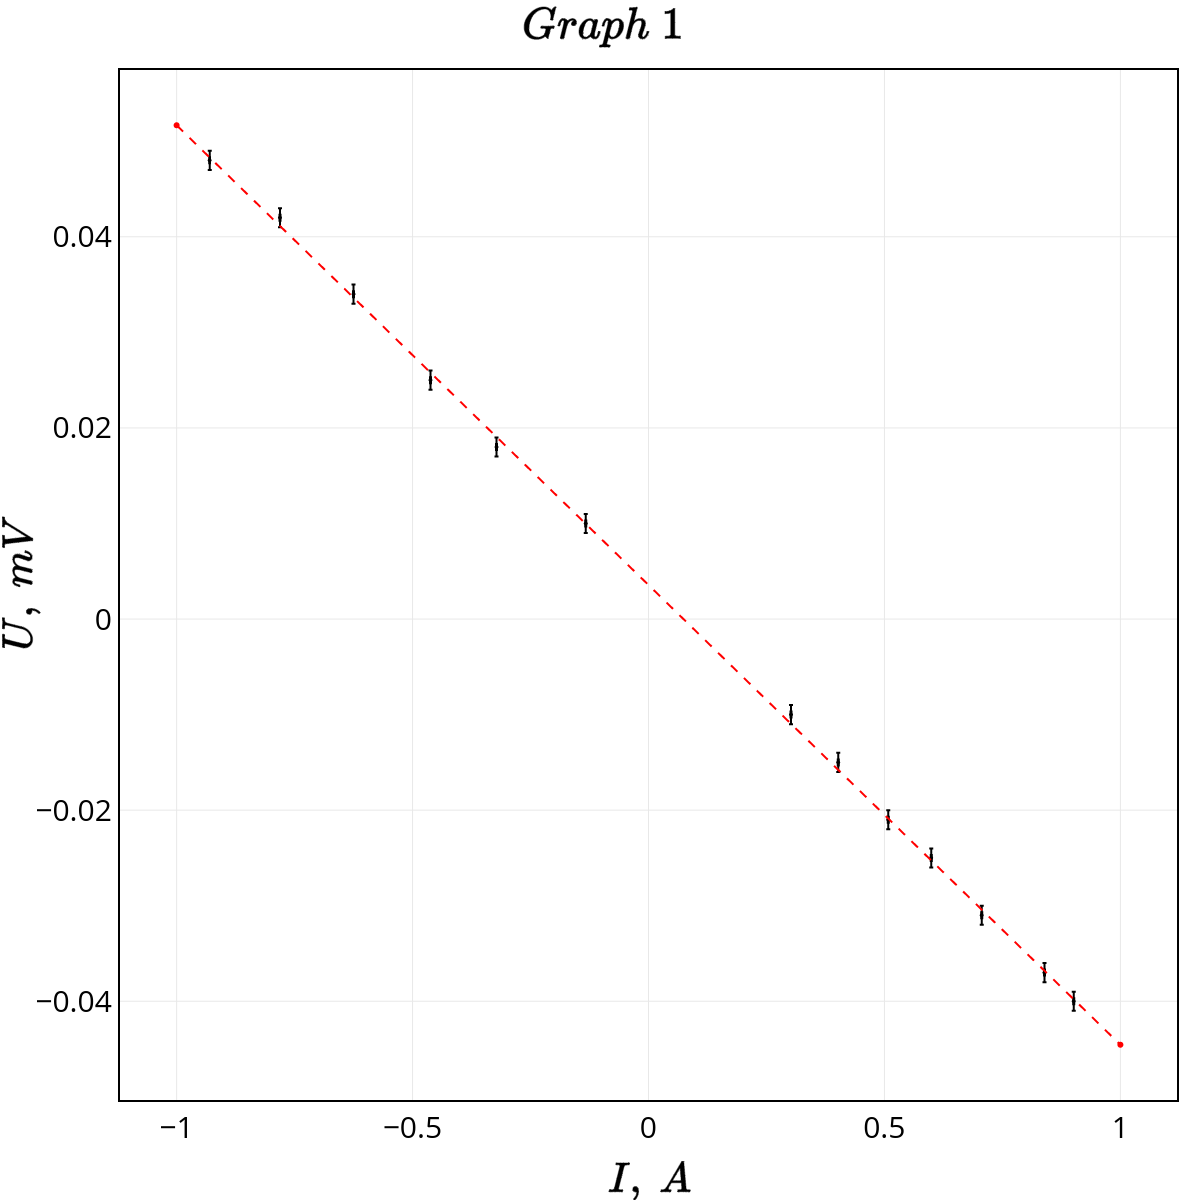
\includegraphics[scale=0.17]{my_plot1.png}}
\end{figure}
\begin{gather*}
R = (4.8 \pm 0.4) \cdot 10^{-5}~\Omega.
\end{gather*}
\item
\textbf{Измерение теплопроводности}\\
Измерим зависимость перепада температур между измерительными точками образца от
выделяемой на нагревателе мощности. Пересчитаем показания вольтметра в температуру,
поделив на коэффициент термопары ($43~mkV/K$) (чувствительность термопары при комнатной температуре). Построим график зависимости $\Delta T(P)$ и по его линейной
модели определим коэффициент $A = l/(\kappa S)$:
\begin{figure}[h]
\center{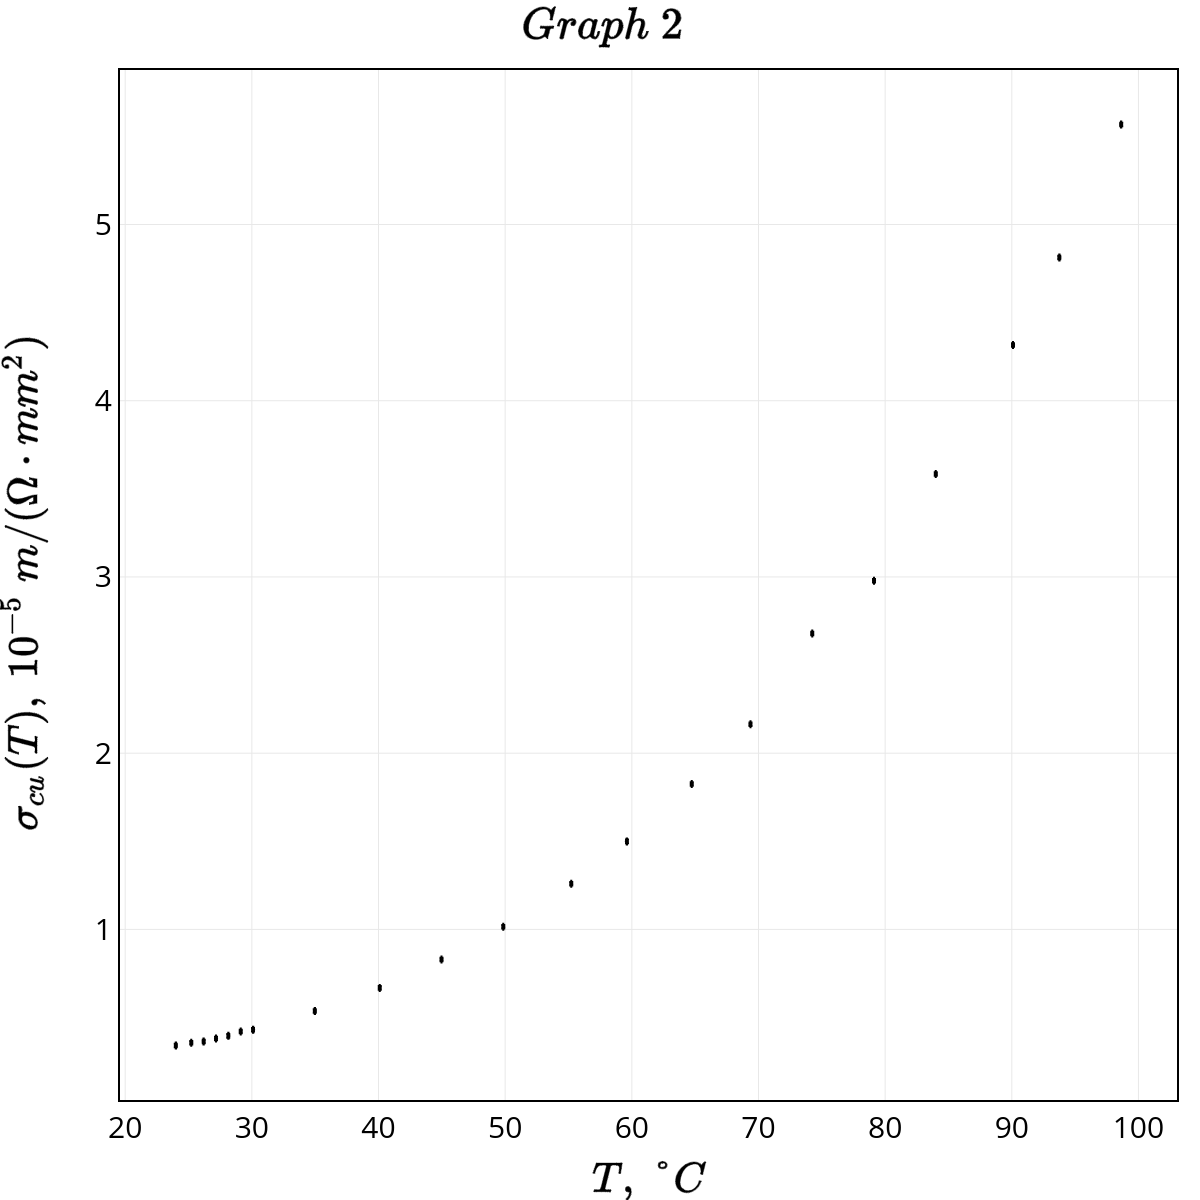
\includegraphics[scale=0.17]{my_plot2.png}}
\end{figure}
\begin{gather*}
A = (5.6 \pm 0.2)~W/K.
\end{gather*}
\item
\textbf{Вычисление числа Лоренца, сравнение с табличным и теоретическим значением}\\
Определим по полученным параметрам постоянную Лоренца для образца №5, взяв среднее
значение для всего набора температур:
\begin{gather*}
L = \frac{\kappa}{\sigma T} = \frac{1}{T}\frac{PR}{\Delta T} =  \frac{1}{T}\frac{R}{A} = \\
= (2.7 \pm 0.3)\cdot 10^{-8} W\cdot\Omega / K^{2}.
\end{gather*}
Рассчитаем теоретическое значение сопротивления и коэффициента теплопроводности для образца №5 (медь, $d = 5~mm$, $l = 50~mm$, $\rho~=~1.65~\Omega \cdot m$, $\kappa = 385~W\cdot m/K)$:
\begin{gather*}
R_{th} = \frac{\rho l}{S} = 4.2 \cdot 10^{-5} \Omega,\\
A_{th} = \frac{l}{\kappa S} = 6.62~W/K,\\
L_{th} = \frac{1}{T}\frac{R}{A} = 2.11\cdot10^{-8}W\cdot\Omega/K^2.
\end{gather*}
Табличное значение постоянной Лоренца при $0^{\circ}C$ и $100^{\circ}C$:
\begin{gather*}
L_{t} = (2.23 - 2.33)\cdot 10^{-8} W\cdot\Omega/K^2.
\end{gather*}
\end{enumerate}
\end{document}